\documentclass{article}
\usepackage{graphicx} % Required for inserting images
\usepackage{verbatim}
\usepackage{amsmath}
\usepackage{algorithmicx}
\usepackage{algpseudocode}
\usepackage{array}
\usepackage{booktabs}
\usepackage{amsmath}
\usepackage{tikz}
\usetikzlibrary{arrows.meta, positioning}


\usepackage{algorithm}



\title{DMA problemset 4}
\author{Daniel Andre Bunckenburg - tvf882@alumni.ku.dk}
\date{February 2025}

\begin{document}

\maketitle


\section*{Problem 1}



\section*{Kosaraju's Algorithm: A Step-by-Step Walkthrough}

We consider a directed graph with vertices
\[
\{a,\, b,\, c,\, d,\, e,\, f,\, g,\, h\}
\]
and edges
\[
a \to b,\quad b \to a,\quad a \to e,\quad b \to c,\quad b \to d,\quad c \to e,\quad c \to f,\quad d \to f,\quad d \to e,
\]
\[
e \to f,\quad e \to h,\quad e \to d,\quad f \to g,\quad g \to h,\quad h \to f,\quad c \to a,\quad a \to d.
\]
Our goal is to find the strongly connected components (SCCs) using Kosaraju’s algorithm.

\section{Step 1: First DFS Pass on the Original Graph}
We perform a depth-first search (DFS) on the original graph to compute finishing times. (Assume we follow the edge order as listed.)

\textbf{Example DFS:}
\begin{enumerate}[label=\textbf{Step \arabic*:}]
    \item \textbf{Start at \(a\):}
    \begin{itemize}
        \item From \(a\), visit \(b\) (via \(a \to b\)).
    \end{itemize}
    
    \item \textbf{At \(b\):}
    \begin{itemize}
        \item \(b \to a\) is skipped (already visited).
        \item Next, \(b \to c\); visit \(c\).
    \end{itemize}
    
    \item \textbf{At \(c\):}
    \begin{itemize}
        \item First, \(c \to e\); visit \(e\).
    \end{itemize}
    
    \item \textbf{At \(e\):}
    \begin{itemize}
        \item \(e \to f\); visit \(f\).
    \end{itemize}
    
    \item \textbf{At \(f\):}
    \begin{itemize}
        \item \(f \to g\); visit \(g\).
    \end{itemize}
    
    \item \textbf{At \(g\):}
    \begin{itemize}
        \item \(g \to h\); visit \(h\).
    \end{itemize}
    
    \item \textbf{At \(h\):}
    \begin{itemize}
        \item \(h \to f\) is skipped (already visited).
        \item Finish \(h\); assign it the earliest finishing time.
    \end{itemize}
    
    \item \textbf{Back to \(g\):}
    \begin{itemize}
        \item No unvisited neighbors; finish \(g\).
    \end{itemize}
    
    \item \textbf{Back to \(f\):}
    \begin{itemize}
        \item Finish \(f\).
    \end{itemize}
    
    \item \textbf{Back to \(e\):}
    \begin{itemize}
        \item Next, \(e \to h\) is skipped (visited), then \(e \to d\); visit \(d\).
    \end{itemize}
    
    \item \textbf{At \(d\):}
    \begin{itemize}
        \item Both \(d \to f\) and \(d \to e\) are already visited.
        \item Finish \(d\).
    \end{itemize}
    
    \item \textbf{Back to \(e\):}
    \begin{itemize}
        \item All edges processed; finish \(e\).
    \end{itemize}
    
    \item \textbf{Back to \(c\):}
    \begin{itemize}
        \item Next, \(c \to f\) and \(c \to a\) are skipped.
        \item Finish \(c\).
    \end{itemize}
    
    \item \textbf{Back to \(b\):}
    \begin{itemize}
        \item Next, \(b \to d\) is skipped.
        \item Finish \(b\).
    \end{itemize}
    
    \item \textbf{Back to \(a\):}
    \begin{itemize}
        \item Next, \(a \to e\) and \(a \to d\) are skipped.
        \item Finish \(a\).
    \end{itemize}
\end{enumerate}

The (hypothetical) finishing times (with larger numbers meaning later finishing) might be:
\[
a: 8,\quad b: 7,\quad c: 6,\quad e: 5,\quad d: 4,\quad f: 3,\quad g: 2,\quad h: 1.
\]
Thus, the order of nodes by decreasing finishing times is:
\[
a,\, b,\, c,\, e,\, d,\, f,\, g,\, h.
\]

\section{Step 2: Reverse the Graph}
We reverse every edge in the graph. For each original edge \( u \to v \), we add an edge \( v \to u \). For example:
\[
a \to b \text{ becomes } b \to a,\quad b \to a \text{ becomes } a \to b,\quad a \to e \text{ becomes } e \to a, \quad \ldots
\]

The reversed graph \( G_R \) (grouped by source) becomes:
\begin{itemize}
    \item \textbf{\(a\)}: \(a \to b\), \(a \to c\) \quad (from \(b \to a\) and \(c \to a\))
    \item \textbf{\(b\)}: \(b \to a\) \quad (from \(a \to b\))
    \item \textbf{\(c\)}: \(c \to b\) \quad (from \(b \to c\))
    \item \textbf{\(d\)}: \(d \to b\), \(d \to e\), \(d \to a\) \quad (from \(b \to d\), \(e \to d\), \(a \to d\))
    \item \textbf{\(e\)}: \(e \to a\), \(e \to c\), \(e \to d\) \quad (from \(a \to e\), \(c \to e\), \(d \to e\))
    \item \textbf{\(f\)}: \(f \to c\), \(f \to e\), \(f \to h\) \quad (from \(c \to f\), \(e \to f\), \(h \to f\))
    \item \textbf{\(g\)}: \(g \to f\) \quad (from \(f \to g\))
    \item \textbf{\(h\)}: \(h \to e\), \(h \to g\) \quad (from \(e \to h\), \(g \to h\))
\end{itemize}

\section{Step 3: Second DFS Pass on the Reversed Graph}
Now, process the nodes in the order of decreasing finishing times from the first DFS. For each unvisited node, perform DFS in the reversed graph to collect an SCC.

\begin{enumerate}[label=\textbf{SCC \arabic*:}]
    \item \textbf{SCC 1:} Start with \(a\) (the highest finishing time).
    \begin{itemize}
        \item Begin Component 1: \(\{a\}\).
        \item From \(a\) in \(G_R\), the neighbors are \(b\) and \(c\).
        \item Visit \(b\) and add it: now \(\{a,\, b\}\).
        \item From \(b\), the neighbor \(a\) is already in the component.
        \item Back at \(a\), visit \(c\) and add it: now \(\{a,\, b,\, c\}\).
        \item From \(c\), the neighbor \(b\) is already in the component.
        \item Finish this component: \(\text{SCC}_1 = \{a,\, b,\, c\}\).
    \end{itemize}
    
    \item \textbf{SCC 2:} Next, the node \(e\) (unvisited).
    \begin{itemize}
        \item Begin Component 2: \(\{e\}\).
        \item From \(e\), the neighbors are \(a\), \(c\), and \(d\). Since \(a\) and \(c\) are already in \(\text{SCC}_1\), visit \(d\) and add it: now \(\{e,\, d\}\).
        \item From \(d\), the neighbors \(b\), \(e\), and \(a\) are already visited.
        \item Finish this component: \(\text{SCC}_2 = \{d,\, e\}\).
    \end{itemize}
    
    \item \textbf{SCC 3:} Next, the node \(f\) (unvisited).
    \begin{itemize}
        \item Begin Component 3: \(\{f\}\).
        \item From \(f\), the neighbors are \(c\), \(e\), and \(h\). Since \(c\) and \(e\) are visited, visit \(h\) and add it: now \(\{f,\, h\}\).
        \item From \(h\), the neighbors are \(e\) and \(g\). \(e\) is already visited; visit \(g\) and add it: now \(\{f,\, h,\, g\}\).
        \item From \(g\), the neighbor \(f\) is already in the component.
        \item Finish this component: \(\text{SCC}_3 = \{f,\, g,\, h\}\).
    \end{itemize}
\end{enumerate}

The remaining nodes (\(g\) and \(h\)) have been visited.

\section*{Final Result}
The strongly connected components (SCCs) of the graph are:
\[
\text{SCC}_1 = \{a,\, b,\, c\},\quad \text{SCC}_2 = \{d,\, e\},\quad \text{SCC}_3 = \{f,\, g,\, h\}.
\]

\section*{Summary}
\begin{itemize}
    \item \textbf{First DFS Pass:} Determines finishing times. For example, we obtained:
    \[
    a: 8,\quad b: 7,\quad c: 6,\quad e: 5,\quad d: 4,\quad f: 3,\quad g: 2,\quad h: 1,
    \]
    so the nodes are processed in the order \(a,\, b,\, c,\, e,\, d,\, f,\, g,\, h\).
    \item \textbf{Graph Reversal:} Every edge is reversed.
    \item \textbf{Second DFS Pass:} Processing nodes in the order from the first pass yielded:
    \begin{enumerate}
        \item Starting at \(a\) produced \(\{a,\, b,\, c\}\).
        \item Next, starting at \(e\) produced \(\{d,\, e\}\).
        \item Then, starting at \(f\) produced \(\{f,\, g,\, h\}\).
    \end{enumerate}
\end{itemize}

This completes the “by hand” run of Kosaraju’s algorithm for the given graph.


\begin{figure}
    \centering
    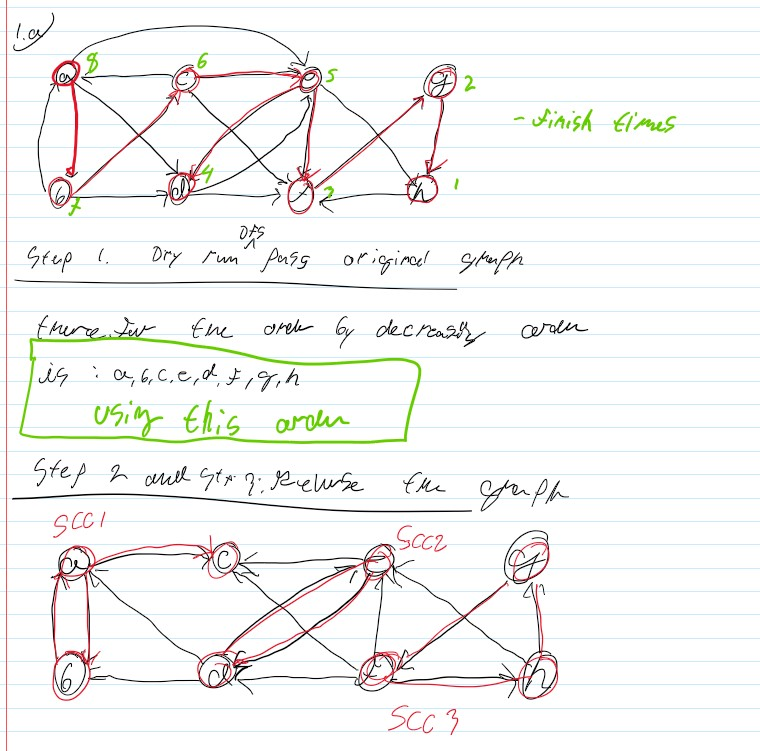
\includegraphics[width=0.5\linewidth]{figures/problemset4_fig_1.jpg}
    \caption{Caption}
    \label{fig:enter-label}
\end{figure}


\section*{Problem 2}


\subsection*{2.1}
\begin{figure}[h!]
    \centering
    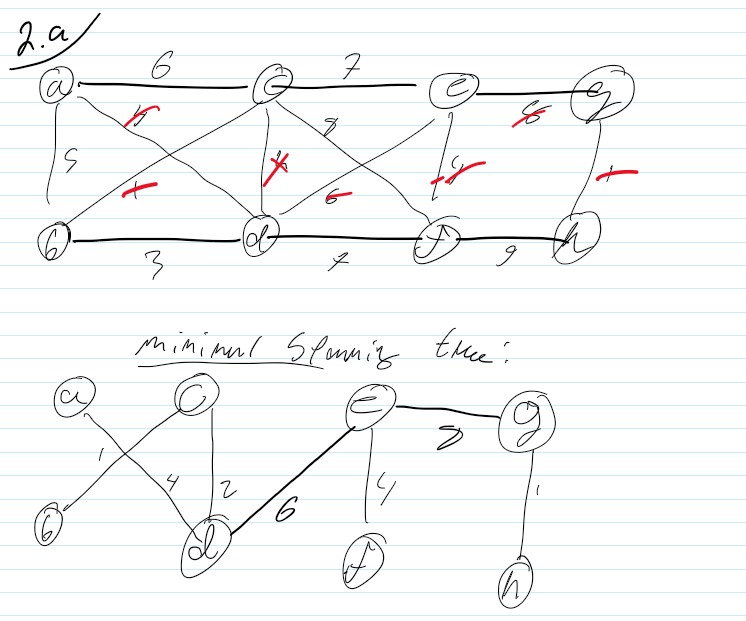
\includegraphics[width=0.5\linewidth]{figures/problemset4_fig_2.jpg}
    \caption{Caption}
    \label{fig:enter-label}
\end{figure}




\subsection*{2.2}

Using the Cut Property, i can say that 


\subsection*{2.3}



\end{document}
